
\chapter{Logiche temporali e model-checking}
\label{Capitolo 6}
Per capire l'importanza di questo argomento pensiamo di avere un codice
concorrente scritto in un certo linguaggio, con l'utilizzo dei \textit{thread},
con un produttore, un consumatore e un buffer. I primi due estendono la classe
\textit{thread} mentre il buffer ha i metodi \textit{synchronized} per il
prelevamento e il deposito. Questo codice simula il modello
produttore-consumatore già approfondito. Bisogna capire se questo programma
funzioni correttamente ma non posso usare le tecniche viste precedentemente per
valutare la correttezza di programmi (logica di Hoare etc$\ldots$) in quanto
abbiamo a che fare con un programma che non inizia, produce dati e finisce ma,
generalmente, si ha a che fare con un programma senza stato finale, che esegue
infinitamente le sue parti in modo concorrente. Per il modello appena ipotizzato
possiamo dire che è corretto se, ad esempio:
\begin{itemize}
  \item ogni oggetto prodotto venga prima o poi consumato
  \item nessun oggetto venga consumato più di una volta
  \item il sistema non vada in deadlock
\end{itemize}
Pensiamo ora ad una rete di Petri ``complessa'' con due processi che
condividono in un mutua esclusione una certa risorsa. Si ha quindi una sezione
critica dove un processo usa tale risorsa. Possiamo volere, per esempio, che i
due processi non siano mai contemporaneamente nella sezione critica (userebbero
insieme la risorsa) e che prima o poi un processo entri in zona critica. Un
metodo è controllare l'intero spazio delle marcature raggiungibili e verificare
che tutto vada come voluto, per la prima richiesta, ma ci sono tecniche
migliori.  \\
Un altro caso d'uso è quello dei circuiti asincroni.\\
Volendo si può adattare la logica di Hoare a modelli concorrenti ma solo se si
ha comunque un output finale e non un'evoluzione ciclica infinita.
\section{Logica PLTL/LTL}
Fino'ora ci si è basati sulla logica proposizionale ma tale logica ha dei
limiti, si introduce quindi la 
\textbf{logica PLTL (\textit{Propositional Linear Time Logic})} che introduce il
concetto di \textbf{tempo}, in ottica \textbf{lineare}, nel processo
logico. Tale logica è anche abbreviata in \textbf{LTL (\textit{Linear Time
    Logic})}.\\  
La logica PLTL viene usata per \textbf{model checking} e lo scopo generale che
ci si propone è quello di presentare un approccio formale alla progettazione e
all'implementazione di sistemi basato su un linguaggio formale che permetta di
specificarli e ragionare sulle loro proprietà. Si vogliono studiare sia sistemi
grandi, come software o addirittura sistemi operativi, che piccoli, come per
esempio una coppia di semafori. Tutti questi sistemi hanno però la medesima
caratteristica, ovvero assumono in ogni \textbf{istante di tempo} un determinato
\textbf{stato} definito dalle \textbf{variabili} del sistema stesso. Si hanno
quindi nel sistema, in ogni istante di tempo:
\begin{itemize}
  \item uno \textbf{stato}, univocamente definito dai valori delle variabili
  \item una \textbf{transizione} che segnala un passaggio da uno stato ad un
  altro
  \item una \textbf{computazione} che rappresenta una sequenza di stati di cui
  ogni coppia forma una transizione. Si introduce quindi il concetto
  \textbf{temporale} 
\end{itemize}
Il \textbf{tempo} viene pensato come un oggetto discreto, cadenzato dalle
transizioni, su cui può essere definita anche una relazione d'ordine (potrebbe
servire che un processo termini prima, dopo o nello stesso tempo di un altro).
\begin{definizione}
  Si definisce \textbf{sistema reattivo} una componente:
  \begin{itemize}
    \item non terminante e interattivo
    \item che può leggere il proprio input non solo all'inizio della
    computazione e che può produrre output non solo alla fine della sua
    computazione (si possono quindi avere multipli input e multipli output)
    \item che interagisce con altri componenti distribuiti o concorrenti
  \end{itemize}
  Sono quindi:
  \begin{itemize}
    \item sistemi concorrenti, distribuiti e asincroni
    \item Non obbediscono al paradigma input-computazione-output
    \item non si possono analizzare con gli strumenti della logica di Hoare
  \end{itemize}
  avendo come esempi di comportamento:
  \begin{itemize}
    \item ``se un messaggio è stato spedito, prima o poi sarà consegnato al
    destinatario''
    \item ``La spia d’allarme resta accesa fino a quando il dispositivo viene
    spento'' 
    \item ``a partire da qualsiasi stato è possibile riportare il sistema allo
    stato iniziale''
  \end{itemize}
\end{definizione}
Bisogna stabilire la correttezza di un sistema reattivo esprimendo il criterio
di correttezza come formula di un opportuno linguaggio logico. Il sistema
reattivo si modella tramite un sistema di transizioni, tramite i \textbf{modelli
di Kripke}, e valutiamo se la formula è vera nel sistema di transizioni, tramite
logiche temporali e algoritmi specifici.\\
Si hanno sistemi non terminanti che usano un numero \textbf{finito} di
variabili e di conseguenza si ha un numero di stati, in cui transita il sistema,
\textbf{finito}. Si hanno infatti sistemi di transizione finiti che
\textit{``comprimono''} sistemi non terminanti, con computazioni di lunghezza
infinita, in una rappresentazione finita.
Si ricorda che si possono inoltre categorizzare le proprietà che vogliamo
specificare come: 
\begin{itemize}
  \item \textbf{proprietà di safety}
  \item \textbf{proprietà di liveness}
  \item \textbf{proprietà di fairness}
\end{itemize}
Introduciamo quindi meglio i \textbf{modelli di Kripke}.\\
\begin{definizione}
  Definiamo un \textbf{sistema di transizioni} $A$ come:
  \[A=(Q, T)\]
  con:
  \begin{itemize}
    \item $Q$ come insieme di stati (potrebbe essere infinito ma studieremo i
    casi finiti)
    \item $T\subseteq Q\times Q$ insieme delle transizioni di stato che portano
    da uno stato ad un altro
  \end{itemize}
\end{definizione}
\begin{definizione}
  Definiamo \textbf{cammino} come:
  \[\pi=q_0q_1q_2\ldots,\,\,\, q_i\in T,\,\,\, \forall\, i\]
  Un cammino può essere infinito.\\
  Definiamo \textbf{cammino massimale} un cammino che non può più essere esteso
  (generalmente studieremo casi dove i cammini massimali sono infiniti).
\end{definizione}
\begin{definizione}
  Definiamo un \textbf{modello di Kripke} $A$ come un sistema di transazioni a
  cui ad ogni stato è associato, dato l'insieme delle proposizioni atomiche
  $AP=\{z_1, z_2,\ldots z_n\}$, un insieme  di
  proposizioni atomiche che sono vere in quello stato:
  \[A=(Q, T, I)\]
  avendo una \textbf{funzione di interpretazione} $I$, che mi restituisce
  l'insieme delle proposizioni atomiche vere in uno stato, tale che:
  \[I:Q\to 2^{AP}\]
  Potrei avere stati dove nessuna proposizione atomica è vera avendo il
  sottoinsieme associato vuoto.\\
  Non si specifica di base uno stato iniziale ma si può arricchire la
  definizione con uno stato iniziale.
\end{definizione}
\begin{esempio}
  Vediamo un esempio:
  \begin{figure}[H]
    \centering
    \begin{tikzpicture}[node distance=2.5cm, bend angle=45, auto]
      \node [place] (p0) [label=below left:q] {1};
      \node [place] (p1) [right of = p0, label=below left:q] {2};
      \node [place] (p2) [right of = p1, label=below left:p] {5};
      \node [place] (p3) [below of = p0, label=below left:{p, r}] {4}; 
      \node [place] (p4) [below of = p1, label=below left:{p, q}] {3}; 
      \node [place] (p5) [below of = p2, label=below left:{p, r}] {6}; 
      \path[-{Latex[width=2mm]}]
      (p0) edge (p1)
      (p1) edge (p2)
      (p1) edge (p4)
      (p4) edge (p3)
      (p3) edge (p0)
      (p2) edge [bend left= 25](p5)
      (p5) edge [bend left= 25](p2)
      ;
    \end{tikzpicture}
  \end{figure}
  Dove:
  \begin{itemize}
    \item $AP=\{p, q, r\}$, insieme delle proposizioni atomiche
    \item $Q=\{1, 2, 3, 4, 5, 6\}$, insieme degli stati (fingiamo che $1$ sia lo
    stato iniziale)
    \item $T=\{(1, 2),(2, 3),(2, 5),(5, 6),(6, 5),\cdots\}$, insieme delle
    transizioni 
    \item $I(4) =\{p, r\}$, $I(2) =\{q\}$ etc$\ldots$, gli altri sono indicati
    in basso a sinistra di ogni stato
    \item $1, 2, 5$ è un cammino non massimale
    \item $1, 2, 5, 6,\overline{5, 6}$ è un cammino massimale (qui indico con la
    linea sopra gli stati in cui poi si continua a ciclare)
    \item $1, 2, 3, 4,\overline{1, 2, 3, 4}$ è un cammino massimale
    \item $1, 2, 3, 4, 1, 2, 5, 6\overline{5, 6}$ è un cammino massimale
  \end{itemize}
\end{esempio}
\begin{definizione}
  Definiamo le famiglie di cammini massimali, indicandole in una notazione tipo
  regex, ($\,^*$ per indicare una o più ripetizione e $\,^\omega$ per indicare
  un ciclo infinito), come le ``tipologie'' di cammino che si possono avere.\\
  (\textit{Il prof non ha davvero dato una definizione})
\end{definizione}
\begin{esempio}
  Nell'esempio sopra si hanno le seguenti famiglie di cammini massimali:
  \begin{itemize}
    \item $(1234)^\omega$
    \item $(1234)^{*}(12)(56)^\omega$
  \end{itemize}
\end{esempio}
Si può quindi già intuire che:
\begin{center}
  \textit{le logiche temporali sono frammenti della logica del primo ordine}
\end{center}
Infatti con le logiche temporali, come la \textit{logica PLTL}, si supera il
limite di rappresentazione temporale della logica proposizionale, permettendo,
per esempio, di rappresentare proposizioni del tipo \textit{``prima o poi'',
  ``accade sempre che'' etc$\ldots$}.\\
Si ha un \textbf{tempo lineare e discreto}, che si può pensare di rappresentare
nella logica classica proposizionale (per esempio come indice) ma questo
comporta il doversi dotare di infinite variabili proposizionali (corrispondenti
ad ogni \textit{``step''} temporale) e comporta l'ottenimento di una formula
proposizionale di lunghezza infinita. Si può pensare di passare allo studio di
questi casi con la \textit{logica predicativa} ma sarebbe ben più del
necessario, in quanto le procedure sarebbero di complessità molto elevata, a
causa della grande espressività della logica predicativa. Inoltre la logica dei
predicati è indecidibile. \\
Si cerca quindi la via di mezzo cercando logiche specializzate, meno espressive
della logica predicativa ma decidibili rispetto ai problemi presi in
considerazione. Si cerca una logica con procedure efficienti rispetto
all'ampiezza della descrizione del problema in analisi (ovvero tipicamente
l'ampiezza del sistema di transizioni), che è direttamente proporzionale al
numero di stati del sistema (lineare rispetto al numero degli stati), e rispetto
alla lunghezza della formula che esprime la proprietà da testare.

\subsection{Sintassi}
Vediamo innanzitutto la \textbf{sintassi} della logica PLTL che chiamiamo anche
LTL.\\
Si ha a che fare con un \textit{vocabolario} più ampio rispetto a quelli della
logica proposizionale, vengono infatti aggiunti dei \textbf{connettivi} utili
alla rappresentazione temporale richiesta.
\begin{definizione}
  Nella logica PLTL, oltre ai connettivi logici classici della logica
  proporzionale, si definiscono i seguenti connettivi:
  \begin{itemize}
    \item \textbf{X}, detto anche \textbf{next} o \textbf{tomorrow}. È un
    connettivo unario e viene rappresentato con $\circ$
    \item \textbf{F}, detto anche \textbf{sometime} o \textbf{future}. È un
    connettivo unario e viene rappresentato con $\diamond$
    \item \textbf{G}, detto anche \textbf{globally} o \textbf{always}. È un
    connettivo unario e viene rappresentato con $\square$
    \item \textbf{U}, detto anche \textbf{until}. È un connettivo binario
  \end{itemize}
  Viene inoltre indicato con $V$ l'\textbf{insieme delle variabili
    proposizionali}, l'\textbf{insieme delle proposizioni atomiche},
  variabili che hanno lo stesso significato della logica
  proposizionale, quindi ogni variabile corrisponde ad una singola proposizione
  del linguaggio naturale. 
\end{definizione}
\textbf{Qui chiamo $V$ quello che prima chiamavo $AP$ per non dover riscrivere
  tutti gli appunti tratti da metodi formali.\\}
\begin{definizione}
  Diamo ora una definizione, formale, procedendo per induzione di
  \textbf{formula ben formata} del linguaggio PLTL (definendo così l'aspetto
  sintattico della logica PLTL): 
  \begin{itemize}
    \item $\forall p\in V$ vale che $p$ è una formula del linguaggio PLTL,
    ovvero le variabili proposizionali della logica classica sono formule del
    linguaggio PLTL. Questa è una \emph{formula atomica}
    \item i simboli $\top$ (detto anche \emph{true} che semanticamente
    semplifica
    una tautologia) e $\bot$ (detto anche \textit{false} o \emph{bottom} che
    semanticamente specifica una formula sempre falsa, ovvero una
    contraddizione) sono formule del linguaggio PLTL. Anche questa è una
    \emph{formula atomica}
    \item se $A$ è una formula del linguaggio PLTL allora lo sono anche:
    \begin{itemize}[label=$\ast$]
      \item $\neg A$
      \item $\mathbf{X}A$
      \item $\mathbf{F}A$
      \item $\mathbf{G}A$
    \end{itemize}
   
    \item  se $A$ e $B$ sono formule del linguaggio PLTL allora lo sono anche:
    \begin{itemize}[label=$\ast$]
      \item $A\to B$
      \item $A\land B$
      \item $A\lor B$
      \item $A\mathbf{U}B$ (anche $\mathbf{U}(A, B)$)
    \end{itemize}
    \item nient'altro appartiene all'insieme delle formule del linguaggio PLTL
  \end{itemize}
  Quindi si nota come \textbf{l'insieme delle formule PLTL contiene quello delle
    formule classiche della logica proporzionale}. Si ha quindi che l'insieme
  delle formule PLTL non è altro che un'estensione di quello delle formule
  classiche della logica proposizionale.
\end{definizione}
Si hanno varianti della logica temporale con anche operatori relativi al passato
ma non sono utili in merito al model checking.
\begin{definizione}
  La sintassi delle formule del linguaggio PLTL possono essere definite usando
  anche la notazione \textbf{BNF (Backus-Naur Form o Backus Normal Form)},
  ovvero, $\forall p\in V$:
  \[A::=p\,|\,\top\,|\,\bot\,|\,(\neg A)\,|\,(A\land A)\,|\,(A\lor A)\,|\,(A\to
    A)\,|\,(\mathbf{X}A)\,|\,(\mathbf{F}A)\,|\,(\mathbf{G}A)\,|\,(A\mathbf{U}A)
  \] 
  Non si è usata quindi una definizione ricorsiva ma viene invece usata una
  \textbf{grammatica}\\
  \begin{shaded}
    La BNF (Backus-Naur Form o Backus Normal Form) è una metasintassi, ovvero un
    formalismo attraverso cui è possibile descrivere la sintassi di linguaggi
    formali (il prefisso meta ha proprio a che vedere con la natura circolare di
    questa definizione). Si tratta di uno strumento molto usato per descrivere
    in modo preciso e non ambiguo la sintassi dei linguaggi di programmazione,
    dei protocolli di rete e così via, benché non manchino in letteratura esempi
    di sue applicazioni a contesti anche non informatici e addirittura non
    tecnologici. La BNF viene usata nella maggior parte dei testi sulla teoria
    dei linguaggi di programmazione e in molti testi introduttivi su specifici
    linguaggi. \\
    In termini formali, la BNF può essere vista come un formalismo per descrivere
    grammatiche libere dal contesto.  \\
    Una specifica BNF è un insieme di regole di derivazione ciascuna espressa
    nella forma: 
    \begin{center}
      \textit{<simbolo> ::= \_espressione\_}
    \end{center}
  \end{shaded}
\end{definizione}
Il cammino nel modello di Kripke corrisponde ad una esecuzione di un sistema,
che è una sequenza di stati. 
\subsection{Semantica}
\begin{definizione}
  La \textbf{semantica}, ovvero il significato dei connettivi della logica PLTL,
  è data usando i cosiddetti \textbf{modelli lineari} (si ricorda l'uso di un
  tempo lineare).\\
  Si consideri una struttura algebrica di questo tipo:
  \[M=\langle S,\,\rho, \,\to, \,\Vdash\rangle\]
  dove:
  \begin{itemize}
    \item $S$ è un \textbf{insieme infinito di stati}, detti anche
    \textbf{mondi}
    \item $\rho \in S$ è uno stato del modello detto anche \textbf{root} o
    \textbf{radice}. In tale stato viene codificato il \textbf{tempo zero}
    \item $\to$ è una relazione binaria su $S$ detta \textbf{relazione di
      transizione} la quale introduce un \textbf{ordinamento lineare} sugli
    elementi di $S$. Si ha quindi che:
    \[\to\,\subseteq S\times S\]
    e, $\forall \alpha \in S$, \textbf{esiste ed è unico} $\beta\in S$ tale che
    vale:
    \[\alpha\to\beta\]
    Preso quindi uno stato qualsiasi ho un solo modo per passare ad un altro
    stato (esiste quindi un ``prima'' e un ``dopo'').\\
    Inoltre vale che, $\forall \alpha\in S$, $\alpha\not\to \rho$, dove $\rho\in
    S$ è l'unico elemento di $S$ a godere di questa proprietà (in quanto $\rho$
    codifica il tempo zero). 
    \item $\Vdash$ è una relazione binaria, inclusa in $S\times V$, detta
    \textbf{relazione di soddisfacibilità}. Solitamente con $\alpha\Vdash p$
    si indica che $(\alpha, p)\in\,\Vdash$ è valido, ovvero che $\alpha$
    \textbf{soddisfa} $p$, con $\alpha\in S$ e $p\in V$
  \end{itemize}
  La struttura $M$ viene detta \textbf{modello per PLTL}.\\
  Si nota come questi modelli lineari seguano un ordinamento simile a quello che
  si ha tra i numeri in $\mathbb{N}$.\\ 
  Si nota come la semantica della logica PLTL sia drasticamente più complessa
  di quella della logica classica proposizionale 
\end{definizione}

Bisogna dare ora significato ai connettivi PLTL. Per i connettivi della logica
proposizionale si usano tavole di verità e induzione ma per la logica PLTL le
cose sono un po' diverse.\\
Per dare un significato alle formule del linguaggio PLTL bisogna basarsi sui
modelli per PLTL.\\

\begin{definizione}
  Vediamo quindi la semantica dei vari operatori.\\
  Diciamo anche che un a formula è vera rispetto ad uno stato $q$ del modello di
  Kripke se è vera in tutti i cammini massimali $\pi$ che partono da $q$,
  dicendo che la formula $\alpha$ è soddisfatta in $\pi$.\\
  Per comodità indichiamo un cammino massimale generico con:
  \[\pi=q_0q_1\ldots q_n\]
  e un suffisso di ordine $i$:
  \[\pi^{(i)}=q_iq_{i+1}\ldots q_j,\mbox{ avendo }\pi=\pi^{(i)}\]
  La formula è vera rispetto ad uno stato $q$ del modello di Kripke se è vera in
  tutti i cammini a partire da $q$.\\
  Si indica con:
  \[\pi\vDash\alpha\]
  per indicare che $\alpha$ è vera/valida in $\pi$ (o che $\pi$ soddisfa
  $\alpha$).\\
  
  Se pensiamo ai modelli di Kripke si ha, dati $\alpha,\beta$ due formule e $p$
  una proposizione atomica:
  \begin{enumerate}
    \item $\pi\vDash p$ sse $p\in I(q_0)$, con $q_0$ stato iniziale scelto
    \item $\pi\vDash \neg \alpha$  sse $\pi\not\vDash \alpha$
    \item $\pi\vDash \alpha\lor\beta$ sse $\pi\vDash \alpha$ o $\pi\vDash \beta$
  \end{enumerate}
  Potenzialmente bastano questi due connettivi per definire tutti gli altri per
  la logica proposizionale. \\
  Passando agli operatori temporali, con $\alpha\in FBF$ (formule ben formate)
  si ha:
  \begin{enumerate}
    \item $\pi\vDash\mathbf{X}\,\alpha$ sse $\pi^{(1)}\vDash \alpha$ (quindi se
    nello stato successivo vale $\alpha$)
    \item $\pi\vDash\mathbf{F}\,\alpha$ sse $\exists
    i\in\mathbb{N}:\pi^{(i)}\vDash  \alpha$ quindi prima o poi $\alpha$ sarà
    vera (quindi può anche essere vera nello stato iniziale con $i=0$)
    \item $\pi\vDash\mathbf{G}\,\alpha$ sse $\forall\, i\in
    \mathbb{N}:\pi^{(i)}\vDash \alpha$, quindi $\alpha$ deve essere vero in
    tutti i suffissi di $\pi$ (e quindi anche nello stato iniziale)
    \item $\pi\vDash\alpha\,\mathbf{U}\,\beta$ sse $\pi^{(i)}\vDash \beta$ (che
    sarebbe $\pi\vDash\mathbf{F}\,\beta$) \textbf{e} $\forall\, h, 0\leq
    h<i,\,\,\, \pi^{(h)}\vDash \alpha$ quindi esiste uno stato $i$ dove vale
    $\beta$ e in tutti gli stati precedenti (escluso $i$) vale $\alpha$. Se
    $\beta$ è vera in $\pi$ posso dire che l'until è valido, trascurando la
    parte dopo l'\textit{and} della formula (modificando la definizione possiamo
    dire che la seconda parte vale solo ``se esistono stati precedenti'').
  \end{enumerate}
\end{definizione}
% \textbf{Vedere anche esempio su slide.}\\
% \begin{esempio}
%   Graficamente si ha qualcosa del tipo:
%   \begin{figure}[H]
%     \centering
%     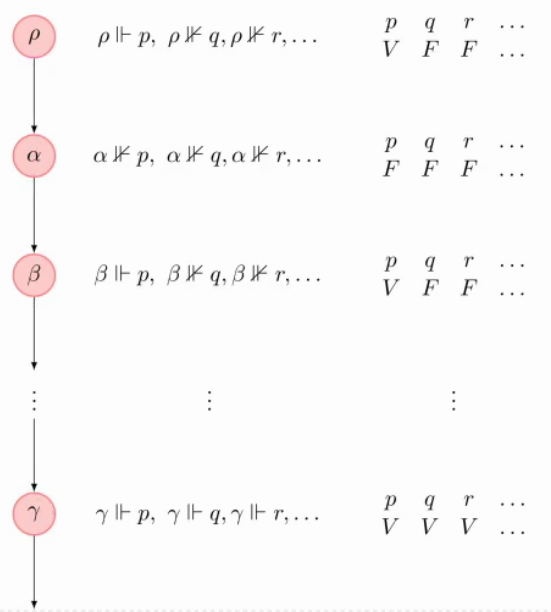
\includegraphics[scale = 0.263]{img/pltl.png}
%   \end{figure}
%   \textbf{che prosegue infinitamente}. Si nota che in ogni stato si specifica
%   se 
%   una variabile proposizionale (che sono infinite) è soddisfatta e, per
%   ciascuna 
%   variabile, si definisce una sorta di \textit{tabella di verità}, che
%   specificare la soddisfacibilità di una variabile in un determinato stato
% \end{esempio}
Si nota che la definizione di \textbf{modello PLTL} non esclude che due stati
diversi possano soddisfare le stesse variabili, ovvero che si possano comportare
nello stesso modo \textit{(come se nulla cambiasse nel tempo)}.
\begin{esempio}
  Vediamo degli esempi (considerando cammini infiniti):
  \begin{itemize}
    \item $\mathbf{FG}\,\alpha$ indica che $\alpha$ è invariante da un certo
    punto in poi
    \item $\mathbf{GF}\,\alpha$ indica che $\alpha$ è vera in un numero infinito
    di stati (ma non necessariamente tutti)
    \item $\mathbf{G}\neq (cs_1\land cs_2)$ è la mutua esclusione, avendo $cs_1$
    e $cs_2$ per indicare che il processo 1 e 2 sono rispettivamente in sezione
    critica 
    \item $\mathbf{G}(req\implies\mathbf{XF}\, ack)$, avendo $req$ richiesta
    pendente di un server e $ack$ aknowledge, per dire che se si ha una
    richiesta pendente prima o poi si avrà il messaggio di ack subito dopo la
    req (non avviene in contemporaneamente ma nello stato dopo)
    \item $\mathbf{G}(req\implies(req\,\mathbf{U}\, ack))$ per dire che è sempre
    vero che se si ha una richiesta da un certo punto in poi si dovrà avere un
    ack, con la req che rimane vera fino al momento prima dell'ack
    \item $\mathbf{G}(req\implies((req\land \neg ack)\,\mathbf{U}\,(ack\land\neg
    req)))$ per dire che se ho una richiesta pendente posso avere che resti tale
    fino all'ack ma quando arriva l'ack la req deve essere ``negativizzata''
    (non serve il next perché tanto non possono valere nello stesso stato per
    come è stata scritta la formula)
  \end{itemize}
\end{esempio}
\begin{esempio}
  Presa la rete:
  \begin{figure}[H]
    \centering
    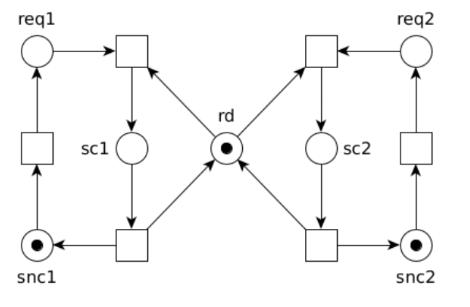
\includegraphics[scale = 0.5]{img/mc.jpg}
  \end{figure}
  con al mutua esclusione, avendo:
  \begin{itemize}
    \item $rd$ la risorsa disponibile
    \item $sc1$ e $sc2$ le due sezioni critiche
    \item $snc1$ e $snc2$ le due sezioni non critiche
    \item $req1$ e $req2$ le due richieste pendenti di usare la risorsa
  \end{itemize}
  avendo il grafo dei casi (ipotizzando per semplicità $1$ come stato iniziale):
  \begin{figure}[H]
    \centering
    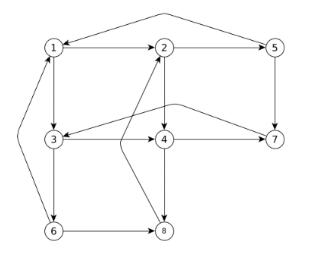
\includegraphics[scale = 0.7]{img/mc2.jpg}
  \end{figure}
  con:
  \begin{itemize}
    \item $1=\{rd, snc1, snc2\}$
    \item $2=\{rd, req1, snc2\}$
    \item $3=\{rd, snc1, req2\}$
    \item $4=\{rd, req1, req2\}$
    \item $5=\{sc1, snc2\}$
    \item $6=\{snc1, sc2\}$
    \item $7=\{sc1, req 2\}$
    \item $8=\{req1, sc2\}$
  \end{itemize}
  che può essere letto come modello di Kripke, con l'elenco sopra che può
  essere visto come la funzione di interpretazione dello stesso.\\
  Studiamo $\mathbf{G}\neq (cs_1\land cs_2)$ e $\mathbf{G}\,(req1\implies
  \mathbf{F}\, sc1)$ (è sempre vero che se vale $req1$ allora prima o poi la
  richiesta verrà soddisfatta).\\
  Per la prima formula possiamo dire che è una \textbf{proprietà di safety},
  esprimendo che non si può raggiungere uno stato ``pericoloso'', come l'uso
  contemporaneo della risorsa. La verifico anche solo scorrendo le
  interpretazioni degli stati e vedendo che non esiste una stato in cui
  compaiono sia $sc1$ che $sc2$ (questo perché ho il globally e basta quindi
  vale semplicemente per tutti gli stati). \\
  Non posso fare lo stesso per la seconda. Ho sempre una globally con quindi
  una proprietà invariante ma ho all'interno un altro operatore temporale
  quindi non posso semplicemente scorrere la lista delle interpretazioni degli
  stati. In ogni caso questa seconda formula non è valida in quando potrei
  avere $(1)(2, 4, 8)^\omega$ in cui anche il secondo processo fa richiesta e ci
  entra. Posso entrare in un loop in cui solamente il processo
  due prende ogni volta la risorsa quindi la formula non è valida in quel
  cammino massimale.\\
  Possiamo comunque trovare cammini in cui vale, come $(1, 3, 6)^\omega$, in
  quanto in quei tre stati $req1$ è sempre falsa.
\end{esempio}
Introduciamo nuovi operatori temporali:
\begin{itemize}
  \item \textbf{weak until}:
  \[\alpha\,\mathbf{W}\,\beta\equiv \mathbf{G}\,\alpha\lor
    (\alpha\,\mathbf{U}\,\beta)\]
  quindi vale se $\alpha$ è sempre vera o se vale l'until classico
  \item \textbf{release}:
  \[\alpha\,\mathbf{R}\,\beta\mbox{ sse }\forall\, k\geq 0:(\pi^{(k)}\vDash
    \beta\lor \exists\, h<k:\pi^{(h)}\vDash \alpha)\]
  ovvero:
  \[\alpha\,\mathbf{R}\,\beta\equiv \beta\,\mathbf{W}\,(\alpha\land \beta)\]
  ovvero vale se $\beta$ è sempre vero o ad un certo punto $\beta$ è vero e
  diventa vero anche $\alpha$ e dall'istante successivo $\beta$ può diventare
  falso. Praticamente $\alpha$ libera $\beta$, che negli istanti successivi può
  essere falsa
\end{itemize}
\textit{Per tradurre un enunciato in linguaggio naturale in logica temporale per
  prima cosa, occorre individuare le proposizioni atomiche; in seguito si
  analizza la struttura della frase, eventualmente riformulandola in una frase
  equivalente con espressioni corrispondentiagli operatori temporali.}\\
\begin{definizione}
  Definiamo l'equivalenza tra due formule come:
  \[\alpha\equiv \beta\iff \forall\,\pi:(\pi\vDash\alpha\leftrightarrow\pi\vDash
    \beta)\]
  per ogni cammino $\pi$. Quindi varia il modo per esprimere la stessa cosa, per
  ogni cammino $\alpha$ è soddisfatta nel cammino sse lo è anche $\beta$ (e
  avendo il sse vale il viceversa).
\end{definizione}
\begin{esempio}
  Vediamo esempi di formule equivalenti:
  \begin{itemize}
    \item $\mathbf{F}\,\alpha\equiv\alpha\lor\mathbf{XF}\,\alpha$\\
    infatti prima o poi diventerà vero $\alpha$ equivale a dire che vale nello
    stato corrente e nello stato prossimo vale che prima o poi sarà vero
    $\alpha$ 
    \item $\mathbf{G}\,\alpha\equiv\alpha\land\mathbf{XG}\,\alpha$\\
    infatti dire che vale sempre $\alpha$ è come dire che ora vale $\alpha$ e
    che nel prossimo stato vale il globally di $\alpha$
    \item $\alpha\mathbf{U}\,\beta\equiv\beta\lor(\alpha\land
    \mathbf{X}\,(\alpha\,\mathbf{U}\,\beta)$ \\
    ovvero l'until è equivalente a dire che ora vale $\beta$ o che ora vale
    $\alpha$ ma nello stato successivo varrà l'until
  \end{itemize}
  Si evidenzia in tutti e tre i casi la natura ricorsiva delle formule della
  logica temporale.\\
  Vediamo infatti altri esempi:
  \begin{itemize}
    \item $\mathbf{FGF}\,\alpha\equiv\mathbf{GF}\,\alpha$
    quindi aggiungere il primo future in \textbf{\textit{FGF}} è inutile
    \item $\mathbf{GFG}\,\alpha\equiv\mathbf{FG}\,\alpha$
    quindi aggiungere il primo globally in \textbf{\textit{GFG}} è inutile   
  \end{itemize}
\end{esempio}

Prendiamo la formula:
\[\top\,\mathbf{U}\,\alpha\]
ma per definizione ci basta dire che $\alpha$ prima o poi diventi vera e
quindi basta:
\[\top\,\mathbf{U}\,\alpha\equiv F\alpha\]
\textbf{Il future può sempre essere rappresentato dall'until}.\\
Vediamo un altra formula:
\[\neg\mathbf{F}\,(\neg\alpha)\]
ma questo equivale a dire:
\[\neg\mathbf{F}\,(\neg\alpha)=\mathbf{G}\,\alpha\]
Quindi il globally può essere derivato dal future che è derivato dall'until e
quindi \textbf{anche il globally potrebbe essere rimosso}.\\
Si può dimostrare che il \textbf{next non è derivabile} e che \textbf{l'until, a
  sua volta, non è derivabile}. 
\begin{definizione}
  Definiamo un \textbf{insieme minale di operatori}. L'insieme
  $\{\mathbf{X},\mathbf{U}\}$ forma un insieme minimale di operatori, dal quale
  possiamo derivare tutti gli altri (\textbf{\textit{F, G, W, R}}).\\
  Potenzialmente potrei quindi usare solo until e next.\\
  Si hanno anche altri insiemi minimali di operatori volendo (ma in tutti ci
  sarà l'until essendo l'unico operatore binario, non potendo derivarlo da uno
  unario). 
\end{definizione}
\noindent
Studiamo ora meglio la negazione di connettivi logici.\\
Pensiamo a ``non è vero che $\mathbf{F}\,\alpha$''. Possiamo riformularla con
``Non è vero che in ogni cammino, prima o poi $\alpha$ diventa vera'', cioè
``esiste un cammino nel quale $\alpha$ è sempre falsa''. D'altro canto
$\neg\mathbf{F}\,\alpha$ significa ``in ogni cammino non è vero che prima o poi
$\alpha$ diventa vera'', che equivale a $\mathbf{G}\,(\neg \alpha)$, quindi in
realtà $\neg\mathbf{F}\,\alpha$ non è la negazione logica di
$\mathbf{F}\,\alpha$ perché nasconde il concetto di ``per ogni cammino'', con
quindi il quantificatore $\forall$. Dalla logica predicativa sappiamo che la
negazione di una formula dove compare un quantificatore equivale a cambiare il
quantificatore e aggiungere la negazione e quindi la riformulazione giusta
sarebbe ``esiste un cammino in cui vale $\mathbf{F}\,\alpha$'', che non può
essere rappresentato in logica temporale LTL (\textbf{CONTROLLARE}). Si ha
quindi un limite 
espressivo, non può esprimere proprietà del tipo:
\begin{center}
  \textbf{\textit{esiste un cammino in cui $\alpha$}}
\end{center}
\begin{esempio}
  Vediamo esempi di proprietà di questo tipo:
  \begin{itemize}
    \item ``è sempre possibile ritornare allo stato iniziale''
    (``è possibile'' si traduce in ``esiste un cammino'')
    \item ``e il processo $P$ chiede la risorsa, è possibile raggiungere uno
    stato di deadlock'' 
  \end{itemize}
\end{esempio}
\begin{esempio}
  Si prenda:
  \begin{figure}[H]
    \centering
    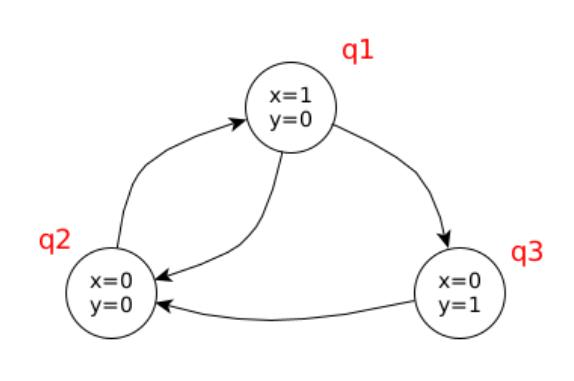
\includegraphics[scale = 0.4]{img/kri.jpg}
  \end{figure}
  che è un modello di Kripke che rappresenta le evoluzioni di un programma con
  due variabili $x$ e $y$. I vari $q_i$ rappresentano i possibili stati.\\
  Studiamo:
  \begin{itemize}
    \item $\mathbf{G}\,(x=0\lor y=0)$
    \item $\mathbf{GF}\,(y=0)$
    \item $\mathbf{GF}\,(y=1)$
    \item $\mathbf{G}\,(x=1\implies \mathbf{F}\,(y=1))$
  \end{itemize}
  per farlo bisogna studiare ogni possibile evoluzione a partire da ogni stato
  (che di volta in volta diventa uno stato iniziale).
  \begin{itemize}
    \item per il primo basta osservare i vari stati e osservare che vale
    l'argomento del globally in ogni stato, quindi qualsiasi sia lo stato
    iniziale varrà il globally (visto che passo in stati in cui vale sempre
    l'argomento) e quindi la formula è verificata
    \item parto dalla formula più interna (dopo aver valutato dove vale
    l'argomento, ovvero in $q_1$ e $q_2$), ovvero il future, e studiare dove
    vale. Per proprietà del future vedo che posso partire da $q_1$ e dire che
    vale (dato che vale anche in $q_1$ stesso), posso partire da $q_2$ per lo
    stesso ragionamento di $q_1$. Ragiono ora su $q_3$, dove non vale $y=0$, ma
    da lui parte un solo arco e porta in uno stato dove vale $y=0$ quindi ogni
    cammino che parte da $q_3$ soddisfa $y=0$. Il future vale quindi in ogni
    stato e di conseguenza anche il globally e quindi la formula è verificata
    \item ragiono come per il caso 2. Per $q_3$ vale ovviamente il future. Passo
    a $q_1$ e già qui vedo che potrei avere un cammino massimale con solo $q_1$
    e $q_2$ e quindi non vale il future. Analogamente si fa lo stesso per $q_2$,
    che non soddisfa il future. Il globally quindi non vale in $q_1$ e $q_2$,
    non valendo lì il future. Studiamo ora $q_3$ ma anche qui non vale in quanto
    potrei, in uno dei cammini da $q_3$ entrare nel loop tra $q_1$ e $q_2$,
    quindi anche per $q_3$ non vale il globally e quindi la formula non è
    verificata    
    \item prendo il cammino che parte da $q_1$ e cicla infinitamente con $q_3$ e
    $q_2$, in questo cammino la formula è verificata. In ogni cammino in qui da
    $q_1$ passo a $q_3$ la formula è verificata ma non lo è nel solito loop tra
    $q_1$ e $q_2$ e quindi la formula non è verificata
  \end{itemize}
\end{esempio}
\begin{esempio}
  Studiamo il modello di Kripke della mutua esclusione:
  \begin{figure}[H]
    \centering
    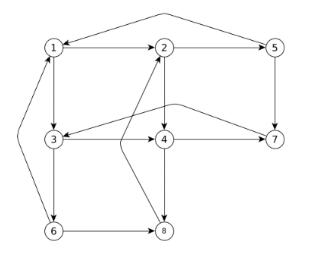
\includegraphics[scale = 0.7]{img/mc2.jpg}
  \end{figure}
  \noindent
  con:
  \begin{itemize}
    \item $1=\{rd, snc1, snc2\}$
    \item $2=\{rd, req1, snc2\}$
    \item $3=\{rd, snc1, req2\}$
    \item $4=\{rd, req1, req2\}$
    \item $5=\{sc1, snc2\}$
    \item $6=\{snc1, sc2\}$
    \item $7=\{sc1, req 2\}$
    \item $8=\{req1, sc2\}$
  \end{itemize}
  avendo:
  \begin{itemize}
    \item $rd$ la risorsa disponibile
    \item $sc1$ e $sc2$ le due sezioni critiche
    \item $snc1$ e $snc2$ le due sezioni non critiche
    \item $req1$ e $req2$ le due richieste pendenti di usare la risorsa
  \end{itemize}
  Si richiede:
  \begin{itemize}
    \item i due processi non sono mai contemporaneamente nella sezione critica
    \item se un processo richiede la risorsa, prima o poi entrerà nella sezione
    critica, escludendo la starvation
    \item se un solo processo richiede la risorsa, deve poter accedere alla
    sezione critica
  \end{itemize}
  Esprimiamo ciò in logica temporale:
  \begin{itemize}
    \item $\mathbf{G}\,\neg(sc1\land sc2)$
    \item $\mathbf{G}\,(req1\implies \mathbf{F}\, sc1)$
    \item non è esprimibile in logica temporale in quanto esprime una
    possibilità 
  \end{itemize}
  Studiamo quindi, informalmente i primi due requisiti:
  \begin{itemize}
    \item la prima proprietà è verificata non avendo stati dove valgono
    contemporaneamente i due argomenti
    \item la seconda non è verificata avendo un cammino massimale
    $(1)(2, 4, 8)^\omega$ che impedisce al primo processo di entrare in sezione
    critica (c'è anche un cammino massimale dove non entra mai il secondo)
  \end{itemize}
  Intuitivamente posso ragionare anche sul terzo requisito possiamo dire che è
  valida in quanto può accedere infinitamente alla risorsa con l'altro che non
  cerca mai di accederci.\\
  Per validare anche la seconda formula possiamo ricordarci l'ultimo accesso e
  in caso di conflitto dare priorità sull'altro accesso. Nel modello di Kripke
  avremmo: 
  \begin{figure}[H]
    \centering
    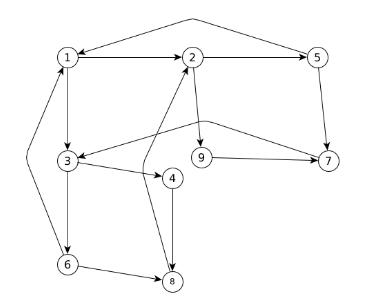
\includegraphics[scale = 0.6]{img/mc3.jpg}
  \end{figure}
  dove lo stato 4 viene sdoppiato in 4 e 9, che hanno le stesse proposizioni
  atomiche, $rd, req1, re2$ ma da entrambi ora parte un singolo arco che
  rispettivamente porta dove l'altro processo è in pending, dandogli poi i
  privilegi di accesso. Si garantisce comunque la mutua esclusione, si soddisfa
  la seconda proprietà (garantendo alternanza di accesso).
\end{esempio}
\section{Computation tree logic}
Studiamo ora \textbf{alberi di computazione} derivati da modelli di Kripke.
\begin{esempio}
  Prendiamo il modello:
  \begin{figure}[H]
    \centering
    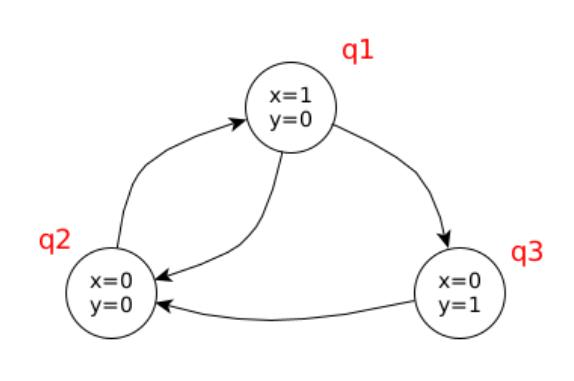
\includegraphics[scale = 0.4]{img/kri.jpg}
  \end{figure}
  Scegliamo come nodo iniziale $q_1$ e costruiamo un albero che rappresenta le
  possibili computazioni:
  \begin{figure}[H]
    \centering
    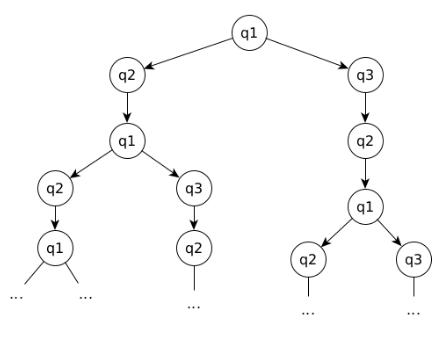
\includegraphics[scale = 0.4]{img/mc4.jpg}
  \end{figure}
\end{esempio}
\begin{definizione}
  Propriamente definiamo \textbf{computazione} un cammino dell'albero a partire
  dalla radice.
\end{definizione}
Passiamo ora alla sintassi delle formule ben formate della \textbf{Computational
  Tree Logic (\textit{CTL})}.
\begin{definizione}
  Si ha che, dato $AP$ insieme delle proposizioni atomiche:
  \begin{itemize}
    \item $\forall p\in AP, p\in FBF$
    \item $\forall\,\alpha,\beta\in FBF$ valgono gli operatori della logica
    proposizionale 
  \end{itemize}
  Aggiungiamo ora i nuovi connettori, \textbf{\textit{A}} e \textit{\textbf{E}},
  che si associano ai connettivi temporali:
  \begin{itemize}
    \item $\mathbf{A}$ indica il ``per ogni cammino''
    \item $\mathbf{E}$ indica il ``esiste almeno un cammino tale che''
  \end{itemize}
  \textbf{Questi operatori possono precedere un solo operatore temporale per
    volta e ogni operatore temporale deve essere preceduto da un
    quantificatore}.\\ 
  Si ha quindi che:
  \begin{itemize}
    \item $\mathbf{AX}\,\alpha,\mathbf{EX}\,\alpha\in FBF$
    \item $\mathbf{AF}\,\alpha,\mathbf{EF}\,\alpha\in FBF$
    \item $\mathbf{AG}\,\alpha,\mathbf{EG}\,\alpha\in FBF$
    \item $\mathbf{A}\,(\alpha\,\mathbf{U}\,\beta),\,\mathbf{E}\,
    (\alpha\,\mathbf{U}\,\beta)\in FBF$    
  \end{itemize}
  Si hanno formule, come $\mathbf{AFG}\,\alpha$, non sono una formula CTL. \\
 \textbf{Si hanno formule LTL che non sono formule CTL, e viceversa}.
\end{definizione}
\textbf{Vari esempi/esercizi su slide del 14 Dicembre.}\\
Si ha che molte proprietà possono essere espresse sia in PLTL che in CTL:
\begin{itemize}
  \item \textbf{proprietà invarianti}, con $\mathbf{G}\,\alpha$ e con
  $\mathbf{AG}\,\alpha$ in CTL
  \item \textbf{proprietà di reattività} (proprietà invarianti condizionali),
  con $\mathbf{G}\,(\alpha\implies \mathbf{F}\,\beta)$ e con
  $\mathbf{AG}\,(\alpha\implies \mathbf{AF}\,\beta)$ in CTL
\end{itemize}
Ma si hanno anche proprietà non rappresentabili. Prendiamo ad esempio la
\textbf{reset property}:
\[\mathbf{AG}\,\mathbf{EF}\,\alpha\]
ovvero \textit{da ogni stato raggiungibile in ogni cammino è sempre possibile
  raggiungere uno stato nel quale vale $\alpha$}. Questa non può essere espressa
in LTL ma solo in CTL.\\
Vediamo una formula che può essere espressa solo in PLTL:
\[\mathbf{FG}\,\alpha\]
ovvero \textit{in ogni cammino, prima o poi si raggiungerà uno statoa partire
  dal quale $\alpha$ rimane sempre vera}. Questa non può essere espressa
in CTL (se prendo l'albero ho cammini in cui non è vero che $\alpha$ rimane
sempre vero) ma solo in PLTL.\\
\textbf{Su slide dimostrazione della cosa tramite confronti}.\\
Si ha un'estensione di CTL e PLTL, detta CTL$^*$, nella quale si mantengono i
quantificatori sui camini ma si elimina il vincolo CTL per il quale ogni
operatore temporale deve avere un quantificatore (posso quindi avere formule del
tipo $\mathbf{EFG}\,\alpha$).\\ 
Potrei avere formule di CTL$^*$ che non sono esprimibili in CTL e
PLTL, estendendone la capacità espressiva ma aumentando la complessità degli
algoritmi associati. In pratica l'insieme delle formule CTL$^*$ contiene gli
altri due (che per di più hanno un'intersezione tra loro).
\section{Model checking}
\begin{definizione}
  Due modelli di Kripke $M_1$ e $M_2$ con stati iniziali $q_0$ e $s_0$, si ha
  che essi sono \textbf{equivalenti} rispetto ad una logica $I$ (che può essere
  PLTL, CTL etc$\ldots$) se, per ogni formula $\alpha\in FBF_I$, si ha:
  \[M_1, q_0\vDash \alpha\iff M_2, s_0\vDash \alpha\]
  Avendo che i due modelli sono effettivamente indistinguibili.\\
  L'equivalenza è quindi in funzione di proprietà della logica stessa.\\
  \textbf{Esempi su slide.}
\end{definizione}
\begin{definizione}
  Si ha che una relazione parziale $\leq$ su $A$:
  \[\leq\,\,\, \subseteq A\times A\]
  è:
  \begin{itemize}
    \item \textbf{riflessiva}, infatti $x\leq x,\,\,\,\forall\, x\in A$ 
    \item \textbf{antisimmetrica}, infatti $(x\leq y\,\,\land\,\, y\leq
    x)\implies  x=y,\,\,\,\forall x, y\in A$
    \item \textbf{transitiva}, infatti $(x\leq y\,\,\land\,\, y\leq z)\implies
    x\leq z,\forall\, x, y, z\in A$
  \end{itemize}
  La notazione:
  \[x<y\]
  significa;
  \[x\leq y\,\,\land\,\, x\neq y\]
\end{definizione}
\begin{definizione}
  Dato $(A,\leq)$ un insieme parzialmente ordinato e $B\subseteq A$ si
  definiscono:
  \begin{itemize}
    \item $x\in A$ è un \textbf{maggiorante} di $B$ se $y\leq
    x,\,\,\,\forall\, y\in B$
    \item $x\in A$ è un \textbf{minorante} di $B$ se $x\leq
    y,\,\,\,\forall\, y\in B$
    \item $B^*$ come \textbf{insieme dei maggioranti di $B$}
    \item $B_*$ come \textbf{insieme dei minoranti di $B$}
    \item $B$ è \textbf{superiormente limitato} se $B^*\neq \emptyset$
    \item $B$ è \textbf{inferiormente limitato} se $B_*\neq \emptyset$
    \item $x\in B$ è il \textbf{minimo} di $B$ se $x\leq y,\,\,\,\forall\, y\in
    B$ 
    \item $x\in B$ è il \textbf{massimo} di $B$ se $y\leq x,\,\,\,\forall\, y\in
    B$
    \item $x\in B$ è il \textbf{minimale} di $B$ se $y\leq x\implies y=x$
    \item $x\in B$ è il \textbf{massimale} di $B$ se $x\leq y\implies y=x$
  \end{itemize}
\end{definizione}
\begin{definizione}
  Si ha che:
  \begin{itemize}
    \item se $x$ è il minimo di $B^*$ allora $x$ è l'\textbf{estremo superiore
      (join)} di $B$:
    \[x=\sup B=\bigvee B\]
    \item se $x$ è il massimo di $B_*$ allora $x$ è l'\textbf{estremo inferiore
      (meet)} di $B$:
    \[x=\inf B=\bigwedge B\]
  \end{itemize}
  In particolare se $B=\{x, y\}$ si ha che $x\lor y$ indica $\bigvee B$ (se
  esiste) e $x\land y$ indica $\bigwedge B$ (se esiste).
\end{definizione}
\begin{definizione}
  Definiamo \textbf{reticolo} un insieme parzialmente ordinato $(L,\leq)$ tale
  che, $\forall\, x, y\in L$ esistono $x\lor y$ e $x\land y$.
\end{definizione}
\begin{definizione} 
  Definiamo \textbf{reticolo completo} se $\bigvee B$ e $\bigwedge B$ esistono
  per ogni $B\subseteq L$.
\end{definizione}
\begin{definizione}
  Prendiamo due insiemi parzialmente ordinati $(A,\leq)$ e $(B,\leq)$, si ha che
  una funzione:
  \[f:A\to B\]
  è detta \textbf{monotona} se, $\forall\, x, y\in A$ vale:
  \[x\leq y\implies f(x)\leq f(y)\]
  ovvero se \textbf{preserva la relazione d'ordine}.\\
  Vale anche nel caso particolare in cui $A$ e $B$ coincidono.
\end{definizione}
\begin{definizione}
  Considerando funzioni con dominio e codominio coincidenti, ovvero del tipo:
  \[f:X\to X\]
  si ha che un elemento $x\in X$ è un \textbf{punto fisso} di $f$ se:
  \[f(x)=x\]
\end{definizione}
\begin{esempio}
  Vediamo qualche esempio:
  \begin{itemize}
    \item $f:\mathbb{R}\to\mathbb{R}$, $f(x)=x^2$ e l'insieme dei punti fissi è
    $\{0, 1\}$ (si nota che la funzione non è monotona)
    \item $f:\mathbb{R}^+\to\mathbb{R}$, $f(x)=\log x$ e l'insieme dei punti
    fissi è $\emptyset$ (si nota che la funzione è monotona)
    \item $f:\mathbb{R}\to\mathbb{R}$, $f(x)=x$ (ovvero l'\textbf{identità}) e
    l'insieme dei punti fissi è $\mathbb{R}$ 
  \end{itemize}
\end{esempio}
Preso un insieme parzialmente ordinato $(A,\leq)$ e $f:A\to A$ monotona. Ci si
chiede se esistono un massimo e un minimo punto fisso.
\begin{esempio}
  Prendiamo $A=2^\mathbb{N}$ e $S\subseteq \mathbb{N}$. Vediamo vari esempi:
  \begin{itemize}
    \item $f(S)=S\cup\{2, 7\}$, una funzione monotona. Si ha che tutti i
    sottoinsiemi che contengono $2$ o $7$ sono punti fissi (ogni insieme delle
    parti di $\{2, 7\}$), tali sottoinsiemi
    sono anche i minimi punti fissi. Si ha un massimo punto fisso che è
    $\mathbb{N}$
    \item $f(S)=S\cap\{2, 7, 8\}$, una funzione monotona. Si ha che il
    sottoinsieme $\{2, 7, 8\}$ è un punto fisso. D'altro canto anche ogni insieme
    appartenente all'insieme delle parti di $\{2, 7, 8\}$ è punto fisso. Il
    massimo punto fisso è $\{2, 7, 8\}$ e come minimo punto fisso abbiamo
    $\emptyset$ 
  \end{itemize}
  Si nota una sorta di simmetria tra massimi e minimi punti fissi nel caso di
  unione o intersezione
\end{esempio}
\begin{esempio}
  Sia $A=\{1,\ldots, 11\}$ visti come stringhe e con questi 11 elementi si
  costruisca un albero binario orientato: 
  \begin{figure}[H]
    \centering
    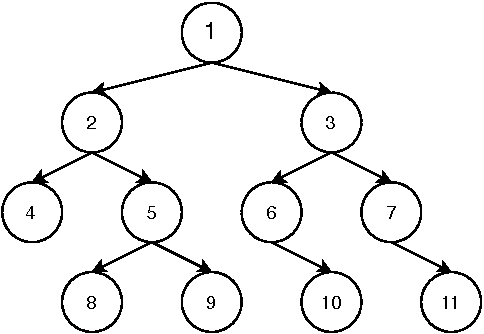
\includegraphics[scale = 0.9]{img/tree.pdf}
  \end{figure}
  Prendiamo l'insieme
  $(\mathcal{P}(A),\subseteq)$ con $\mathcal{P}$ che indica l'insieme delle
  parti.\\
  Si ha:
  \[f:\mathcal{P}(A)\to \mathcal{P}(A)\]
  con:
  \[F(S))S\cup\{x\in A|x\mbox{ è figlio di un }y\in S\}\]
  ad esempio:
  \[f(\{2, 6\})=\{2, 6, 4, 5, 10\}\]
  quindi $f(\{2, 6\})$ non è un punto fisso.\\
  Si ha anche che:
  \[f(\{2, 6, 4, 5, 10\})=\{2, 6, 4, 5, 10, 8, 9\}=M\]
  Ma quindi:
  \[f(M)=M\qquad f(\emptyset)=\emptyset\]
  I punti fissi di questa funzione sono i cosiddetti \textbf{insiemi chiusi
    verso il basso}, ovvero un insieme che se contiene un certo nodo contiene
  anche tutti i discendenti di quel nodo (ovvero tutti i sottoalberi
  discendenti).\\
  Il massimo punto fisso è $A$ stesso mentre il minimo punto fisso è l'insieme
  vuoto (ed esistono vari punti fissi minimali).
  \label{es:k}
\end{esempio}
\begin{teorema}[di Knaster-Tarski]
  Sia $(L,\leq)$ un reticolo completo (quindi per ogni coppia si hanno
  \textit{join} e \textit{meet} e quindi ogni sottoinsieme finito di elementi di
  $L$ ha ancora \textit{join} e \textit{meet}, anche i sottoinsiemi infiniti) e
  $f:L\to L$ una funzione monotona. Si ha 
  in tal caso che $f$ ha un punto fisso minimo e un punto fisso massimo.\\
  Detto altrimenti l'insieme dei punti fissi forma un reticolo completo (e
  quindi necessariamente si ha un minimo e un massimo).\\
  \textbf{Riascolare esempio detto prima della pausa}.
\end{teorema}
\begin{proof}
  Per semplicità consideriamo $L=\mathcal{P}(A)$ per un certo insieme $A$,
  sapendo che l'insieme delle parti è un reticolo completo (nonché un'algebra
  booleana).\\
  Sappiamo che $f:2^A\to 2^A$ (con $2^A$ che è $\mathcal{P}(A)$ è monotona.\\
  Costruiamo l'insieme:
  \[\mathcal{Z}=\{T\subseteq A|\, f(T)\subseteq T\}\]
  Chiamiamo gli elementi di $\mathcal{Z}$ \textbf{punti pre-fissi}. Si ha che
  $\mathcal{Z}$ non può essere vuoto qualsiasi sia $A$ (se reticolo) e qualsiasi
  sia $f$ (se monotona) in quanto contiene almeno gli elementi di $A$.\\
  Poniamo che $f$ abbia dei punti fissi. Si ha che $\mathcal{Z}$ conterebbe
  tutti questi punti fissi. \\
  Diciamo che:
  \[m=\bigcap \mathcal{Z}\]
  e si ha che $m\subseteq A$ ($m$ potrebbe essere $\emptyset$).\\
  Si ha che $\forall S\in \mathcal{Z}$ $m\subseteq S$ e , per la monotonia: 
  \[f(m)\subseteq f(S)\]
  ma quindi si ha che:
  \[f(m)\subseteq f(S)\subseteq S\]
  Quindi ogni immagine di $m$ è contenuta in $S$.\\
  Possiamo quindi dire che è contenuto nell'intersezione degli elementi di
  $\mathcal{Z}$: 
  \[f(m)\subseteq\bigcap \mathcal{Z}=m\]
  e quindi:
  \[m\in \mathcal{Z}\]
  e quindi $m$ è il minimo di $\mathcal{Z}$ (che non ha nemmeno elementi
  minimali che non contengono $m$). Quindi:
  \[m=\min\mathcal{Z}\]
  Quindi manca da dimostrare che $m$ sia un punto fisso.\\
  Ripartiamo da:
  \[f(m)\subseteq m\]
  avendo una relazione d'ordine tra due sottoinsiemi di $A$. MA avendo che $f$ è
  monotona posso dire che:
  \[f(f(m))\subseteq f(m)\]
  e quindi $f(m)\in \mathcal{Z}$. Ma si ha anche che $m\subseteq f(m)$, avendo
  che $m=\min\mathcal{Z}$. Possiamo quindi concludere che:
  \[m=f(m)\]
  e quindi è un punto fisso.\\
  Concludendo abbiamo visto che $m$ è minimo ed è un punto fisso.\\
  Il ragionamento si può fare analogo e speculare per il massimo punto fisso.\\
  \textbf{Riascoltare dimostrazione}
\end{proof}
\begin{esempio}
  Riprendendo l'esempio \ref{es:k}, avendo una funzione monotona avendo dominio
  e codominio che sono reticoli completi (un reticolo finito è sempre completo),
  so sicuramente che ci sono un punto fisso massimo e uno minimo.
\end{esempio}
Questo teorema è poco utile dal punto di vista algoritmico, dovendo costruire
$\mathcal{Z}$ che può essere infinito.\\
Per lo più il model checking si fa su insiemi finiti ma con un numero di stati
magari enorme e quindi analizzare tutti i sottoinsiemi è poco pratico. Si ha
quindi un altro teorema.
\begin{teorema}[di Kleene]
  Sia $f:2^A\to 2^A$ una funzione monotona. Tale funzione è \textbf{continua}
  se, con $X_i\subseteq 2^A$:
  \[X_1\subseteq X_2\subseteq\cdots\subseteq X_i\subseteq\cdots\]
  e si prendano le immagini:
  \[f(X_1)\subseteq f(X_2)\subseteq\cdots\subseteq f(X_i)\subseteq\cdots\]
  Possiamo dire che:
  \[f\left(\bigcup X_i\right)=\bigcup f(X_i)\]
  Questa proprietà non è detto che valga se la funzione è solo monotona ma deve
  essere anche continua e in tal caso si ha che:
  \begin{itemize}
    \item il minimo punto fisso di $f$ (che esiste per il teorema precedente)
    può essere calcolato con:
    \[f(\emptyset),\qquad f(f(\emptyset)),\qquad f(f(f(\emptyset))),
      \qquad\cdots\]
    calcolando lo ``step'' successivo fino ad arrivare ad un punto fisso
    arrivando prima o poi al minimo punto fisso 
    \item il massimo punto fisso di $f$ (che esiste per il teorema precedente)
    può essere calcolato con:
    \[f(A),\qquad f(f(A)),\qquad f(f(f(A))),\qquad\cdots\]
    arrivando prima o poi al massimo punto fisso (occhio che $A$ è quello di
    $2^A$) 
  \end{itemize}
\end{teorema}
\begin{esempio}
  Siano $A=2^{\mathbb{N}}$, $S\subseteq\mathbb{N}$ e $F(S)=S\cup \{2, 7\}$.\\
  Applico $f$ all'insieme vuoto e trovo $\{2, 7\}$ che non è punto fisso e quindi
  proseguo. Applico poi a $\{2, 7\}$ e ritrovo $\{2, 7\}$ che quindi è un punto
  fisso ed è il minimo. Per il massimo al primo step arrivo a dire che
  $\mathbb{N}$ è il massimo punto fisso (\textbf{non chiaro perché parte da
    $\mathbb{N}$ e non da $2^{\mathbb{N}}$}).  
\end{esempio}
\begin{esempio}
  \textbf{Su slide disegni dell'esempio.}\\
  Si supponga di avere un modello di Kripke e si vuole risolvere il model
  checking globale per $\mathbf{F}\, p$.\\
  Aggiungiamo tutti gli stati in cui in un solo step arriviamo sicuramente in
  uno stato dove vale $p$. \\
  Ora rifacciamo aggiungendo gli stati dove con uno step arriviamo sicuramente
  in uno stato dove vale $p$ o dove vale che allo step successivo sicuramente
  vale $p$. Procedo aumentando di volta in volta l'insieme ``buono'' fino a che
  non possiamo aggiungere nulla. Abbiamo trovato un minimo punto fisso
  dell'algoritmo. \\
  Valuto ora $\mathbf{G}\, p$ e ragiono all'inverso di come fatto prima
  escludendo di volta in volta gli stati in cui non vale $\mathbf{G}\, p$ (quindi
  l'insieme di partenza, diciamo, è quello in cui vale $\neg p$). Di volta in
  volta escludo gli stati che mi portano ad avere $\neg p$ più gli eventuali
  stati già inclusi nell'insieme in uno step precedente fino a che non ho più
  passi possibili. Si arriva a trovare il massimo punto fisso.
\end{esempio}
\begin{definizione}
  Definiamo \textbf{automi di B\"{u}chi} come automi finiti che riconoscono
  parole infinite su un alfabeto $\Sigma$. Si indicano con la quadrupla:
  \[B=(Q, q_0,\delta, F)\]
  con:
  \begin{itemize}
    \item $Q$ insiemi di stati, detti \textit{locations}
    \item $q_0\in Q$ stato iniziale
    \item $\delta\subseteq Q\times \Sigma\times Q$ relazione di transizione
    \item $F\subseteq Q$ insieme di stati accettanti (non si può dire finali in
    quanto le stringhe sono infinite)
  \end{itemize}
  Presa quindi una parola infinita:
  \[w=a_0a_1\cdots\]
  essa è accettata da $B$ se la sequenza di stati corrispondente $q_0q_1\cdots$
  passa infinite volte per almeno uno stato di $F$. In altri termini mi fermo se
  uno stato non ha un arco uscente che porta alla lettera successiva altrimenti
  mi sposto in quello stato ma non serve che mi fermo in uno stato accettante ma
  è sufficiente passarci infinite volte.\\
  Diciamo che $L(B)$ è il linguaggio, ovvero l'insieme di tutte le parole
  accettate dalla'automa.
\end{definizione}
\begin{teorema}
  Il problema:
  \[L(B)=\emptyset\]
  è \textbf{decidibile}.
\end{teorema}
\begin{esempio}
  Sia:
  \begin{center}
    \begin{tikzpicture}[shorten >=1pt, node distance=2cm, on grid, auto]
      \node[state, initial, accepting] (q_0) {$q_0$};
      \node[state] (q_1) [right=of q_0] {$q_1$};
      \path[->]
      (q_0) edge  [bend left = 25]node {$a$} (q_1)
      (q_1) edge  [bend left = 25]node {$b$} (q_0)
      (q_0) edge [loop above] node {$b$} (q_0)
      (q_1) edge [loop above] node {$a$} (q_1)
      ;
    \end{tikzpicture}
  \end{center}
  Si ha:
  \begin{itemize}
    \item $w_1=bbbbbbbbb\cdots$ che è accettata
    \item $w_2=bbaaabbbb\cdots$ che è accettata
    \item $w_3=babababab\cdots$ che è accettata
    \item $w_4=baabbbaaa\cdots$ che non è accettata
  \end{itemize}
\end{esempio}
\begin{esempio}
  Studiamo la formula $\mathbf{GF}\, p$ e sia:
   \begin{center}
    \begin{tikzpicture}[shorten >=1pt, node distance=2cm, on grid, auto]
      \node[state, initial] (q_0) {$q_0$};
      \node[state, accepting] (q_1) [right=of q_0] {$q_1$};
      \path[->]
      (q_0) edge  [bend left = 25]node {$\{p\}$} (q_1)
      (q_1) edge  [bend left = 25]node {$\emptyset$} (q_0)
      (q_0) edge [loop above] node {$\emptyset$} (q_0)
      (q_1) edge [loop above] node {$\{p\}$} (q_1)
      ;
    \end{tikzpicture}
  \end{center}
  Immaginiamo qualche computazione:
  \begin{itemize}
    \item $w_1=\emptyset\{p\}\{p\}\emptyset\{p\}\emptyset\emptyset\cdots$ che
    non è accettata 
    \item $q_2=\emptyset\{p\}\emptyset\{p\}\emptyset\{p\}\emptyset\cdots$ che è
    accettata 
  \end{itemize}
  
\end{esempio}
Possiamo associare ad una computazione su un modello di Kripke una parola che
viene eseguita su un certo automa di di B\"{u}chi.\\
Un automa di B\"{u}chi corrisponde quindi ad una formula PLTL, ma bisogna notare
che l'insieme degli stati dell'automa non ha una relazione diretta con il
modello di Kripke.\\
Vediamo quindi l'algoritmo per vedere se una formula $\alpha$ è vera in
$(M, q_0)$:
\begin{itemize}
  \item costruiamo l'automa che verifica quando $\alpha$ non è verificata
  $B_{\neg\alpha}$ (non dimenticando i discorsi fatti in merito alla negazione
  in PLTL)
  \item trasformiamo $M$ in un automa etichettato come $B_{\neg\alpha}$ ovvero
  in un automa etichettato da insiemi diproposizioni atomiche 
  \item calcoliamo il prodotto sincrono dei due automi, che chiamiamo $PS$. Dati
  due automi definiti sullo stesso alfabeto il prodotto sincrono è un automa che
  corrisponde ad eseguire in parallelo i due automi in modo che procedano con le
  stesse etichette. Gli stati sono quindi il risultato del prodotto cartesiano
  tra gli stati dei due automi
  \item se $L(PS)=\emptyset$ allora $M, q_0\vDash\alpha$, in quando nel modello
  di Kripke $M$ non c'è nessun cammino infinito nel quale non è verificata
  $\alpha$, che quindi è valida nel modello di Kripke. Altrimenti si potrebbe
  eseguire un cammino in $M$ in cui non sarebbe soddisfatto $\alpha$ (si genera
  in caso anche un controesempio in cui la formula $\alpha$ è violata)
\end{itemize}
Passiamo ora cercare un algoritmo per CTL.
\begin{definizione}
  Fissiamo $M=(Q, T, I)$ e sia $\alpha$ una formula. Si definisce
  \textbf{estensione di $\alpha$}:
  \[[[\alpha]]=\{q\in Q|\, M, q\vDash \alpha\}\]
  Se $\alpha=\top$ estensione è l'insieme di tutti gli stati, se è $\bot$ è
  l'insieme vuoto. Se la formula è una proposizione atomica allora l'estensione
  è l'insieme degli stati dove vale la proposizione atomica. Se ho un connettivo
  tra due formule già estese segue la logica dell'operatore (esempio se ho l'and
  in un certo stato è valido sse valgono entrambe le proposizioni).\\
  Passiamo a CTL.\\
  Sia $\alpha\equiv\mathbf{AF}\,\beta$. Si
  definisce la funzione:
  \[f_\alpha:2^Q\to 2^Q\]
  ovvero una funzione che prende un sottoinsieme di stati e lo trasforma in un
  sottoinsieme di stati. Si ha che $\forall H\subseteq Q$:
  \[f_\alpha(H)=[[\beta]]\cup\{q\in Q|\forall(q, q')\in T:q'\in H\}\]
  Si noti che $f_a(\emptyset)=[[\beta]]$.\\
  Si dimostra che $[[\alpha]]$ è il minimo punto fisso di $f_\alpha$.\\
  Ogni volta si aggiungono nuovi stati.\\
  Posso usare lo stesso algoritmo per vedere se $\alpha$ vale in un certo stato,
  osservando se alla fine lo stato che ci interessa è contenuto
  nell'estensione.\\
  Sia ora $\alpha\equiv \mathbf{EG}\,\beta$. Si
  definisce la funzione:
  \[g_\alpha:2^Q\to 2^Q\]
  Si ha che $\forall H\subseteq Q$:
  \[g_\alpha(H)=[[\beta]]\cap\{q\in Q|\exists(q, q')\in T:q'\in H\}\]
  Si noti che $g_\alpha(Q)=[[\beta]]$.\\
  Si dimostra che $[[\alpha]]$ è il massimo punto fisso di $g_\alpha$.\\
  Ogni volta si tolgono stati.\\
  In generale si nota che il ``per ogni'' e l' ``esiste'' compaiono nella
  formula.\\
  Per l'operatore next è sufficiente guardare il passo successivo quindi non
  serve un ragionamento così complesso mentre per l'until si fa un ragionamento
  simile al future, essendo nella pratica una sua forma rafforzata (poi si
  cerca, come per il future, il minimo punto fisso).
\end{definizione}
Possiamo quindi trovare un algoritmo per CTL che sarà ricorsivo.
\begin{definizione}
  Definiamo \textbf{$\mu$ calcolo} come un linguaggio logico che permette di
  definire formule ricorsive.  
\end{definizione}
Si supponga di avere solo l'operatore temporale next e i
quantificatori. Cerchiamo di esprimere, solo con il next, la proprietà
$\mathbf{EF}\,\alpha$. Si ha quindi una sorta di srotolamento:
\[\mathbf{EF}\,\alpha\equiv \alpha\lor
  \mathbf{EX}\,\alpha\lor\mathbf{EXEX}\,\alpha\lor\cdots\]
che è una formula infinita ma con una struttura ben definita, dal secondo
termine si inizia sempre con $\mathbf{EX}$. Raccogliamo:
\[\mathbf{EF}\,\alpha\equiv \alpha\lor
  \mathbf{EX}(\,\alpha\lor\mathbf{EX}\,\alpha\lor\cdots)\]
ma quindi tra parentesi si ha in pratica la formula completa di
$\mathbf{EF}\,\alpha$ e quindi posso dire che:
\[\mathbf{EF}\,\alpha\equiv\alpha\lor\mathbf{EX}\,(\mathbf{EF}\,\alpha)\]
Fisso quindi una notazione per scrivere questa cosa:
\[\mu Y.(\alpha\lor \mathbf{EX}\, Y)\]
Dove la $\mu$ indica tradizionalmente il minimo punto fisso, Quindi la formula
si legge ``minimo punto fisso della funzione $(\alpha\lor \mathbf{EX}\, Y)$ dove
$Y$ è l'oggetto che cerchiamo di definire''. È quindi una forma compatta di
scrivere la formula infinita.\\
Passo a $\mathbf{AG}\alpha$:
\[\mathbf{AG}\,\alpha\equiv \alpha\land
  \mathbf{AX}\,\alpha\land\mathbf{AXAX}\,\alpha\land\cdots\]
e quindi, raccogliendo:
\[\mathbf{AG}\,\alpha\equiv\alpha\land \mathbf{AX}\,(\mathbf{AG}\alpha)\]
ovvero:
\[\nu Y.(\alpha\land\mathbf{AX}\, Y)\]
Possiamo generalizzare fino ad avere un linguaggio completo, una nuova logica,
detto appunto \textbf{calcolo $\mu$}.
\begin{definizione}
  Dato $AP$ l'insieme delle proposizioni atomiche e siano $\alpha$ e $\beta$ due
  formule. Si ha che la sintassi del linguaggio è:
  \begin{itemize}
    \item $\alpha\lor\beta$ e $\neg \alpha$ sono formule (forse anche le altre
    ottenute con connettivi logici (???))
    \item $\mathbf{AX}\,\alpha$ e $\mathbf{AX}\,\alpha$ sono formule
    \item $\mu Y.f(Y)$ è una formula è una formula, dove $f$ è una formula nella
    quale compare $Y$ (con restrizioni sulle negazioni) 
    \item $\nu Y.f(Y)$ è una formula è una formula, dove $f$ è una formula nella
    quale compare $Y$ (con restrizioni sulle negazioni)
  \end{itemize}
  Si ha quindi un modo molto libero di costruire formule.\\
  La semantica del calcolo $\mu$ è definita sui modelli di Kripke attraverso gli
  operatori di punto fisso, usando idee simili a quelle usate per definire le
  estensioni di formule temporali.
\end{definizione}
Si nota che:
\[CTL^*\subset \mbox{calcolo } \mu\]
quindi tutte le formule di $CTL^*$ sono esprimibili nel $\mu$ calcolo che quindi
è più espressivo di tutte le logiche finora considerate (ed esprime anche cose
che le altre non possono). La massima potenza espressiva si paga in complessità
degli algoritmi e con una sorta di ``oscurità'' delle formule, che non sono
facilmente leggibili ed interpretabili.\\
Vediamo qualche dettaglio sulla complessità temporale, dato un modello di
Kripke $M$ e una formula $f$, a parità di algoritmo canonico:
\begin{itemize}
  \item PLTL ha complessità $O(|M|\cdot 2^{|f|})$
  \item CTL ha complessità $O(|M|\cdot |f|)$
\end{itemize}
In realtà la dimensione della formula rende difficile un confronto diretto in
quanto una proprietà può avere una formula breve in LTL e una lunga in CTL (come
abbiamo già visto). Anche il numero di stati, $|M|$, è da non trascurare in
quanto può essere immenso, anche dal punto di vista della complessità
spaziale. Si hanno quindi strategie per la trattazione 
efficiente, tra cui:
\begin{itemize}
  \item rappresentazioni simboliche, tramite diagrammi di traduzione
  binari (Ordered Binary Decision Diagrams, OBDD)
  \item partial order reduction (tramite unfolding), spesso usato per le
  reti di Petri. SI hanno tecniche efficienti dal punto di vista spaziale
  \item traduzione in SAT, usando i SAT solver
\end{itemize}
Quindi, per concludere, per fare model checking una tecnica è ridurre il
problema ad un modello di kripke.\\
Parliamo giusto un secondo di \textbf{fairness}.
\begin{definizione}
  Si dice che un'esecuzione è \textbf{unfair} se un evento rimane sempre
  abilitato da un certo istante in poi ma non scatta mai.\\
\end{definizione}
\begin{definizione}
  Si definisce \textbf{fairness debole} se un evento che è abilitato
  prima o poi scatta o viene disabilitato.
\end{definizione}
Bisogna quindi limitare la valutazione di una formula alla sua esecuzione
\textbf{fair}, nella realtà è irrealistico pensare che qualcosa non scatti
mai essendo sempre abilitata.
\begin{definizione}
  Si definisce \textbf{fairness forte} se ogni evento che viene abilitato
  infinite volte scatta infinite volte (a lungo termine senza curarsi degli
  aspetti quantitativi). Ovvero, in PLTL, se:
  \[\mathbf{GF}\,(\mbox{evento è abilitato})\to\mathbf{GF}\,(\mbox{evento
      scatta})\] 
\end{definizione}
\textbf{Su slide vari esempi per la fairness.}\\
Per il model checking si hanno diversi tool, tra cui:
\begin{itemize}
  \item \textbf{Spin} per PLTL, tramite un linguaggio chiamato Promela
  \item \textbf{NuSMV} per PLTL e CTL
  \item \textbf{mCLR2} per il $\mu$ calcolo
  \item \textbf{TiNA} per PLTL e reti di Petri
\end{itemize}